

\documentclass[12pt]{article}
\usepackage{amsmath}
\usepackage{latexsym}
\usepackage{amsfonts}
\usepackage[normalem]{ulem}
\usepackage{array}
\usepackage{amssymb}
\usepackage{graphicx}
\usepackage[backend=biber,
style=numeric,
sorting=none,
isbn=false,
doi=false,
url=false,
]{biblatex}\addbibresource{bibliography.bib}

\usepackage{subfig}
\usepackage{wrapfig}
\usepackage{wasysym}
\usepackage{enumitem}
\usepackage{adjustbox}
\usepackage{ragged2e}
\usepackage[svgnames,table]{xcolor}
\usepackage{tikz}
\usepackage{longtable}
\usepackage{changepage}
\usepackage{setspace}
\usepackage{hhline}
\usepackage{multicol}
\usepackage{tabto}
\usepackage{float}
\usepackage{multirow}
\usepackage{makecell}
\usepackage{fancyhdr}
\usepackage[toc,page]{appendix}
\usepackage[hidelinks]{hyperref}
\usetikzlibrary{shapes.symbols,shapes.geometric,shadows,arrows.meta}
\tikzset{>={Latex[width=1.5mm,length=2mm]}}
\usepackage{flowchart}\usepackage[paperheight=11.0in,paperwidth=8.5in,left=1.18in,right=1.18in,top=0.98in,bottom=0.98in,headheight=1in]{geometry}
\usepackage[utf8]{inputenc}
\usepackage[T1]{fontenc}
\TabPositions{0.49in,0.98in,1.47in,1.96in,2.45in,2.94in,3.43in,3.92in,4.41in,4.9in,5.39in,5.88in,}

\urlstyle{same}




% 1) Section
% 1.1) SubSection
% 1.1.1) SubSubSection
% 1.1.1.1) Paragraph
% 1.1.1.1.1) Subparagraph


\setcounter{tocdepth}{5}
\setcounter{secnumdepth}{5}





\setlistdepth{9}
\renewlist{enumerate}{enumerate}{9}
		\setlist[enumerate,1]{label=\arabic*)}
		\setlist[enumerate,2]{label=\alph*)}
		\setlist[enumerate,3]{label=(\roman*)}
		\setlist[enumerate,4]{label=(\arabic*)}
		\setlist[enumerate,5]{label=(\Alph*)}
		\setlist[enumerate,6]{label=(\Roman*)}
		\setlist[enumerate,7]{label=\arabic*}
		\setlist[enumerate,8]{label=\alph*}
		\setlist[enumerate,9]{label=\roman*}

\renewlist{itemize}{itemize}{9}
		\setlist[itemize]{label=$\cdot$}
		\setlist[itemize,1]{label=\textbullet}
		\setlist[itemize,2]{label=$\circ$}
		\setlist[itemize,3]{label=$\ast$}
		\setlist[itemize,4]{label=$\dagger$}
		\setlist[itemize,5]{label=$\triangleright$}
		\setlist[itemize,6]{label=$\bigstar$}
		\setlist[itemize,7]{label=$\blacklozenge$}
		\setlist[itemize,8]{label=$\prime$}

\setlength{\topsep}{0pt}\setlength{\parskip}{8.04pt}
\setlength{\parindent}{0pt}




\renewcommand{\arraystretch}{1.3}






\begin{document}
\begin{Center}
{\fontsize{14pt}{16.8pt}\selectfont \textbf{EV\_2\_4\_GIRO\_DE\_UN\_MOTOR\_DE\_CORRIENTE\_DIRECTA}\par}
\end{Center}\par

\begin{Center}
\textit{SISTEMAS ELECTRÓNICOS DE INTERFAZ}
\end{Center}\par


\vspace{\baselineskip}




\begin{figure}[H]
	\begin{Center}
		
\includegraphics[width=5.24in,height=6.06in]{./media/image1.png}
	\end{Center}
\end{figure}


\par

\begin{Center}
\textbf{Nombre:} Giovanni Daniel Ruiz Tinoco
\end{Center}\par

\begin{Center}
\textbf{Grupo y carrera: }4-B Ing. Mecatrónica
\end{Center}\par

\begin{Center}
\textbf{Profesor: }Carlos Enrique Morán Garabito
\end{Center}\par


\vspace{\baselineskip}

\vspace{\baselineskip}

\vspace{\baselineskip}
\newpage
\begin{justify}
{\fontsize{14pt}{16.8pt}\selectfont \textbf{Giro de un motor en CD}\par}
\end{justify}\par

\begin{justify}
Se trata de hacer girar un motor de corriente continua en los dos sentidos posibles de giro (derecha o izquierda). Primero veremos los esquemas y luego la construcción de un sencillo conmutador con \href{https://www.areatecnologia.com/materiales/madera.html}{madera} y una punta que nos permitirá hacer el cambio de giro del motor de una forma barata, práctica y sencilla.\\
\\
Un motor cambia de sentido de giro cuando cambia la polaridad en su bornes (contactos)
\end{justify}\par



%%%%%%%%%%%%%%%%%%%% Figure/Image No: 2 starts here %%%%%%%%%%%%%%%%%%%%

\begin{figure}[H]
	\begin{Center}
		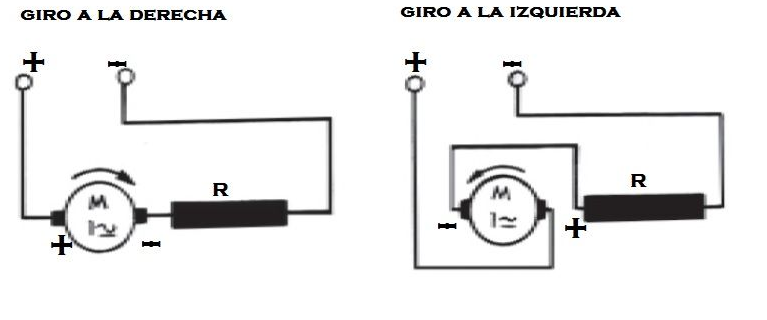
\includegraphics[width=6.14in,height=2.56in]{./media/image2.png}
	\end{Center}
\end{figure}


%%%%%%%%%%%%%%%%%%%% Figure/Image No: 2 Ends here %%%%%%%%%%%%%%%%%%%%

\par

\begin{justify}
De esta forma tendríamos que cambiar la instalación para que girara en un sentido o en otro. Esto no es nada práctico. Lo que queremos conseguir es un esquema con el que podamos cambiar el sentido de giro mediante interruptores o mediante un simple conmutador, y sin cambiar la instalación.
\end{justify}\par



%%%%%%%%%%%%%%%%%%%% Figure/Image No: 3 starts here %%%%%%%%%%%%%%%%%%%%

\begin{figure}[H]
	\begin{Center}
		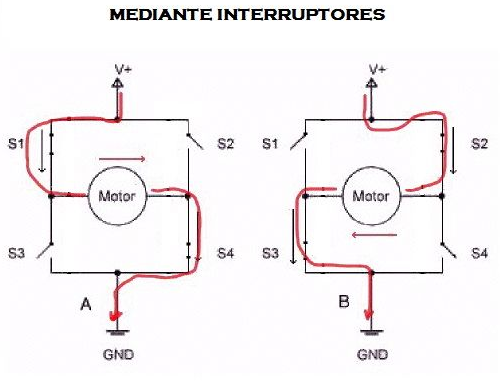
\includegraphics[width=4.32in,height=3.29in]{./media/image3.png}
	\end{Center}
\end{figure}


%%%%%%%%%%%%%%%%%%%% Figure/Image No: 3 Ends here %%%%%%%%%%%%%%%%%%%%

\par

\begin{Center}
\textbf{\textit{Esquemas más comunes de la inversión del sentido de giro de las conexiones de un motor C.C más habituales}}
\end{Center}\par



%%%%%%%%%%%%%%%%%%%% Figure/Image No: 4 starts here %%%%%%%%%%%%%%%%%%%%

\begin{figure}[H]
	\begin{Center}
		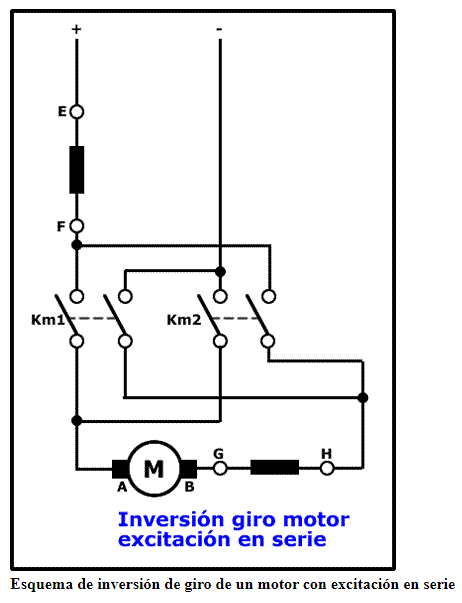
\includegraphics[width=3.26in,height=4.26in]{./media/image4.png}
	\end{Center}
\end{figure}


%%%%%%%%%%%%%%%%%%%% Figure/Image No: 4 Ends here %%%%%%%%%%%%%%%%%%%%

\par



%%%%%%%%%%%%%%%%%%%% Figure/Image No: 5 starts here %%%%%%%%%%%%%%%%%%%%

\begin{figure}[H]
	\begin{Center}
		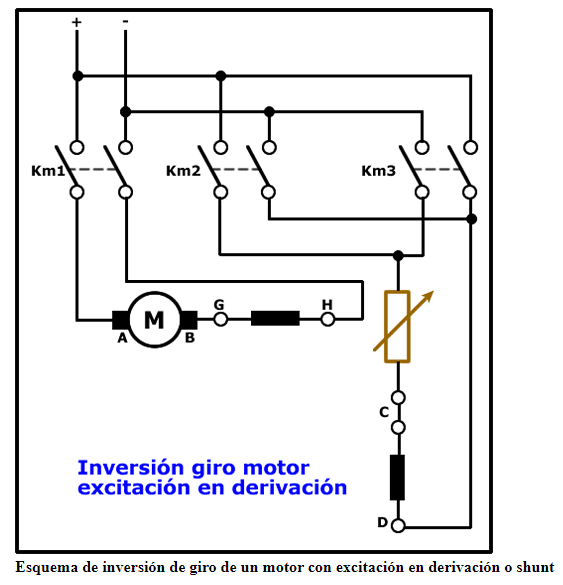
\includegraphics[width=3.32in,height=3.45in]{./media/image5.png}
	\end{Center}
\end{figure}


%%%%%%%%%%%%%%%%%%%% Figure/Image No: 5 Ends here %%%%%%%%%%%%%%%%%%%%

\par


\printbibliography
\end{document}